
%(BEGIN_QUESTION)
% Copyright 2015, Tony R. Kuphaldt, released under the Creative Commons Attribution License (v 1.0)
% This means you may do almost anything with this work of mine, so long as you give me proper credit

A very common form of transformer used in industrial control circuits is the {\it control power transformer}, shown in both pictorial and schematic forms.  Most commonly, the primary winding actually consists of {\it two} coils which may be connected in different ways depending on the amount of voltage available from the AC power source:

$$\includegraphics[width=15.5cm]{i00267x01.eps}$$

Determine first how 240 VAC power would be connected to the primary winding terminals.  After this, determine how a higher line voltage of 480 VAC power would be connected to the primary winding terminals.

\vskip 10pt

Next, identify how a multimeter could be used to test the windings of this transformer, both for {\it open} as well as {\it shorted} faults.

\vskip 10pt

Finally, determine how you would use a piece of test equipment called an {\it insulation tester} (often referred to by the brand name ``Megger'') to check the transformer windings for a short to ground (to the iron core of the transformer), and how this particular type of test equipment differs from a regular ohmmeter.


\vskip 20pt \vbox{\hrule \hbox{\strut \vrule{} {\bf Suggestions for Socratic discussion} \vrule} \hrule}

\begin{itemize}
\item{} Explain why the H2/H3 terminals are ``crossed over'' as they are shown in the schematic diagram.
\item{} Determine how this transformer could be re-designed to provide two different secondary voltage options (240 VAC vs. 120 VAC) as well as two different primary voltage options.
\end{itemize}

\underbar{file i00267}
%(END_QUESTION)





%(BEGIN_ANSWER)

$$\includegraphics[width=15.5cm]{i00267x02.eps}$$

I'll let you determine ways to use a multimeter for winding tests in a control power transformer.

\vskip 10pt

A {\it megger} is a special high-resistance ohmmeter using a test voltage of several hundred or thousand volts.  It is able to detect faults in the insulation of transformer windings in the multiple-megaohm range!

%(END_ANSWER)






%(BEGIN_NOTES)

In order to detect an {\it open} fault, you must measure high resistance between points which should be connected (e.g. between H1-H2, between H3-H4, between X1-X2).

\vskip 10pt

In order to detect a {\it shorted} fault, you must measure abnormally low resistance between points (e.g. between H1-H2, between H3-H4, between X1-X2, between any terminal and the iron core).

%INDEX% Electronics review: megger (test equipment)
%INDEX% Troubleshooting review: electric circuits

%(END_NOTES)


